\documentclass{beamer}
\usepackage{ctex}
\usetheme{AnnArbor}
\usecolortheme{spruce}
\usepackage[utf8]{inputenc}
\usepackage{fontspec}
\usepackage{xeCJK}
\usepackage{graphicx}
\usepackage {mathtools}
\usepackage{utopia}

\setbeamerfont{headline}{family=\kaishu}
\setbeamerfont{footline}{family=\kaishu}
\setbeamerfont{frametitle}{family=\kaishu}

%----------

\definecolor{myNewColorA}{RGB}{0, 81, 40}
\definecolor{myNewColorB}{RGB}{153, 193, 173}
\definecolor{myNewColorC}{RGB}{216, 232, 224}
\setbeamercolor*{palette primary}{bg=myNewColorC}
\setbeamercolor*{palette secondary}{bg=myNewColorB, fg = white}
\setbeamercolor*{palette tertiary}{bg=myNewColorA, fg = white}
\setbeamercolor*{titlelike}{fg=myNewColorA}
\setbeamercolor*{title}{bg=myNewColorA, fg = white}
\setbeamercolor*{item}{fg=myNewColorA}
\setbeamercolor*{caption name}{fg=myNewColorA}
\usefonttheme{professionalfonts}
\usepackage{natbib}
\usepackage{hyperref}
\hypersetup{
	colorlinks=true,
	linkcolor=black,
	citecolor=black
}

%----------

\titlegraphic{
\includegraphics[height=1.5cm]{hzau-logo.eps}}
\setbeamertemplate{background}{
\includegraphics[width=12.8cm]{background.jpg}}

%----------

\setbeamerfont{title}{size=\large}
\setbeamerfont{subtitle}{size=\small}
\setbeamerfont{author}{size=\small}
\setbeamerfont{date}{size=\small}
\setbeamerfont{institute}{size=\small}
\author[张子栋]{张子栋}
\title[枯草芽孢杆菌群比较基因组分析]{枯草芽孢杆菌群比较基因组分析}
\subtitle{中期检查答辩}
\institute[HZAU CoI]{华中农业大学
	
	信息学院}
\date[2024.3.23]{2024年3月23日}

%----------

\AtBeginSection[]
{
	\begin{frame}{}
		\transfade
		\tableofcontents[sectionstyle=show/shaded,subsectionstyle=show/shaded/hide]
		\addtocounter{framenumber}{0}
	\end{frame}
}

%----------

\begin{document}
	\kaishu
	
	\frame{\titlepage}
	
	\begin{frame}
		\frametitle{目录}
		\tableofcontents
	\end{frame}
	
	\section{引言}

	\begin{frame}{引言}
		\qquad 微生物作为地球上最古老、最丰富的生命形式之一,对生态系统的平衡和人类生活产生了深远的影响。21 世纪,高通量测序技术我们能够直接从环境样本中获取微生物群落的遗传信息,进行更深入的解读研究。

		\qquad 对微生物进行比较基因组学研究能进一步揭示微生物的遗传多样性,发现新的基因和功能。此外,对微生物分类和系统发育研究也有一定的促进作用。

		\qquad 枯草芽孢杆菌在农业生产、水产养殖以及人体健康等方面有着各种积极作用,本人毕业论文将从比较基因组学方面对枯草芽孢杆菌进行较深入的分析。
	\end{frame}

	\section{材料与方法}
	\subsection{材料}
	\begin{frame}{材料与方法}{材料}
		\qquad 研究数据从 NCBI 下载,包括 390 个枯草芽孢杆菌全基因组。

		\begin{figure}
			\centering
			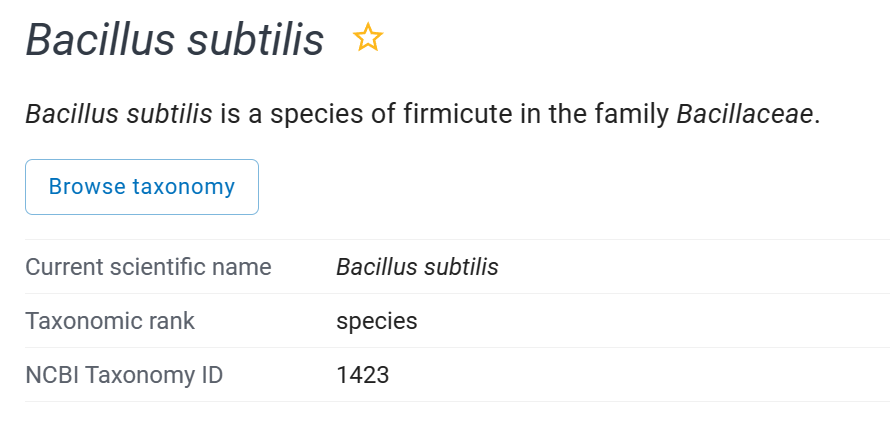
\includegraphics[width=0.8\textwidth]{figure/NCBI.png}
		\end{figure}
	\end{frame}

	\subsection{方法}
	\begin{frame}{材料与方法}{方法}
		根据比较基因组学的一般流程,本人论文将从以下几个方面展开:
		\begin{enumerate}
			\item 基因组组分分析
				\begin{itemize}
					\item Glimmer \& Prodigal
				\end{itemize}
			\item 基因功能分析
				\begin{itemize}
					\item GO Annotation
					\item KEGG Annotation
					\item CAZy Annotation
				\end{itemize}
			\item 泛基因组分析
				\begin{itemize}
					\item Core Gene
				\end{itemize}
			\item 比较基因组分析
				\begin{itemize}
					\item 系统发育树
					\item 共线性分析
				\end{itemize}
		\end{enumerate}
	\end{frame}

	\section{目前进度}
	\begin{frame}{目前进度}{}
		\qquad 目前已经完成基因组组分分析和
	\end{frame}

	\begin{frame}{目前进度}{过程记录}
		\qquad 实验过程均以 Markdown 文档记录,并使用 Git 进行版本管理,有助于后续整理出完成的比较基因组分析流程。

		\quad \\

		GitHub 地址:
	\end{frame}

	\section{后续研究步骤}
	\begin{frame}{后续研究步骤}{待完成步骤}
		\begin{itemize}
			\item 泛基因组分析
			\item 比较基因组分析
		\end{itemize}
		
	\end{frame}

	

	\begin{frame}{后续研究步骤}{结果解读与可视化}
		除去既定方法中的剩余步骤外,还有以下部分需要完成:
		\begin{enumerate}
			\item 结果数据解读
			\item 生物信息学意义分析
			\item 结果可视化
		\end{enumerate}
	\end{frame}

	\section*{致谢}  
	\begin{frame}
		\begin{center}
			\textcolor{myNewColorA}{\huge {谢谢!\\ \quad \\ 请老师批评指正!}}
		\end{center}
	\end{frame}
	
\end{document}